\section{Оценка эффективности}
В рамках оценки эффективности разработанного программного комплекса проведём несколько серий экспериментов с его помощью, а затем осуществим анализ экспериментальных данных.

Далее в этом разделе мы последовательно рассмотрим следующие серии экспериментов и их анализ:
\begin{itemize}
    \item серия экспериментов по проверке точности измерения времени;
    \item серия экспериментов по сравнению производительности программ, собранных компиляторами GCC и LLVM на настройках «по умолчанию»;
    \item группа серий экспериментов по моделированию и предсказанию производительности программы из набора Polybench на различном аппаратном обеспечении:
    \begin{itemize}
        \item серия экспериментов по моделированию и предсказанию производительности при размере входных данных, который меняется по степенному закону, а обе размерности входных данных одинаковы;
        \item серия экспериментов по моделированию и предсказанию производительности при размере входных данных, который меняется случайно при равномерном распределении случайной величины, а обе размерности входных данных одинаковы;
        \item серия экспериментов по моделированию и предсказанию производительности при размере входных данных, который меняется случайно при равномерном распределении случайной величины, а размерности входных данных не одинаковы.
    \end{itemize}
\end{itemize}

\subsection{Серия экспериментов по проверке точности измерения времени}
\label{series-accuracy}
Для проверки точности измерения времени проведём следующий эксперимент.

Сгенерируем семейство программ, которые не делают ничего, кроме вызова функции стандартной библиотеки \textit{C} \texttt{usleep}. Аргументами функции будет число $10^n$, где $n$ --- число от одного до шести включительно. Таким образом, после запуска программа устанавливает таймер на заданное число микросекунд (от 1 мкс до 1000000 мкс = 1 с), останавливается и после его срабатывания завершает работу.

Далее на рис. \ref{img:calibration} приведён график измеренного времени исполнения семейства таких программ и «реального» времени их выполнения --- т.е. времени, указанного в аргументе функции, создающей таймер. График построен с помощью инструментария в автоматическом режиме.

\begin{figure}[p]
    \center{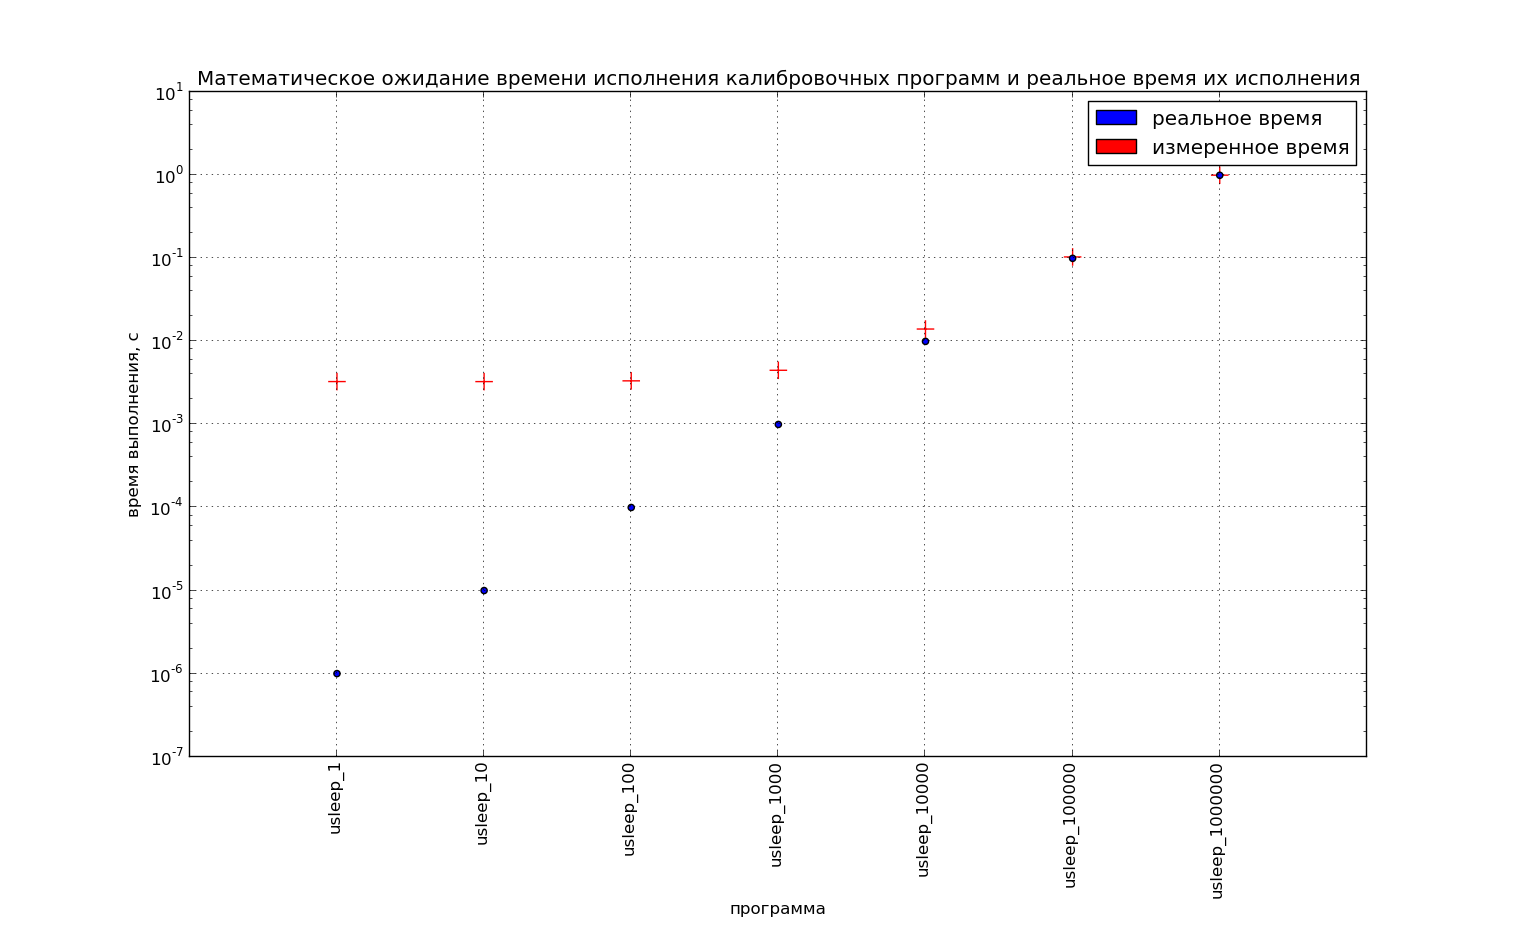
\includegraphics[width=1\linewidth]{calibration}}
    \caption{График измеренного и реального времени исполнения семейства калибровочных программ}
    \label{img:calibration}
\end{figure}

Как мы видим на рис. \ref{img:calibration}, измеренное время асимптотически приближается к значению между $10^{-2}$ и $10^{-3}$ --- около 0,005.

Из этого можно сделать вывод, что существуют постоянные расходы на запуск программы из нашей системы и их можно вычесть из измеренного времени для повышения точности измерения. Для этого мы вычисляем время выполнения пустой программы (согласно описанной в подразделе~\ref{sssect:calibration} методике), а затем вычитаем его из каждого измеренного результата выполнения реальных программ.

На рис. \ref{img:calibration-offset} показан график измеренного времени в данном эксперименте с учётом накладных расходов.

\begin{figure}[p]
    \center{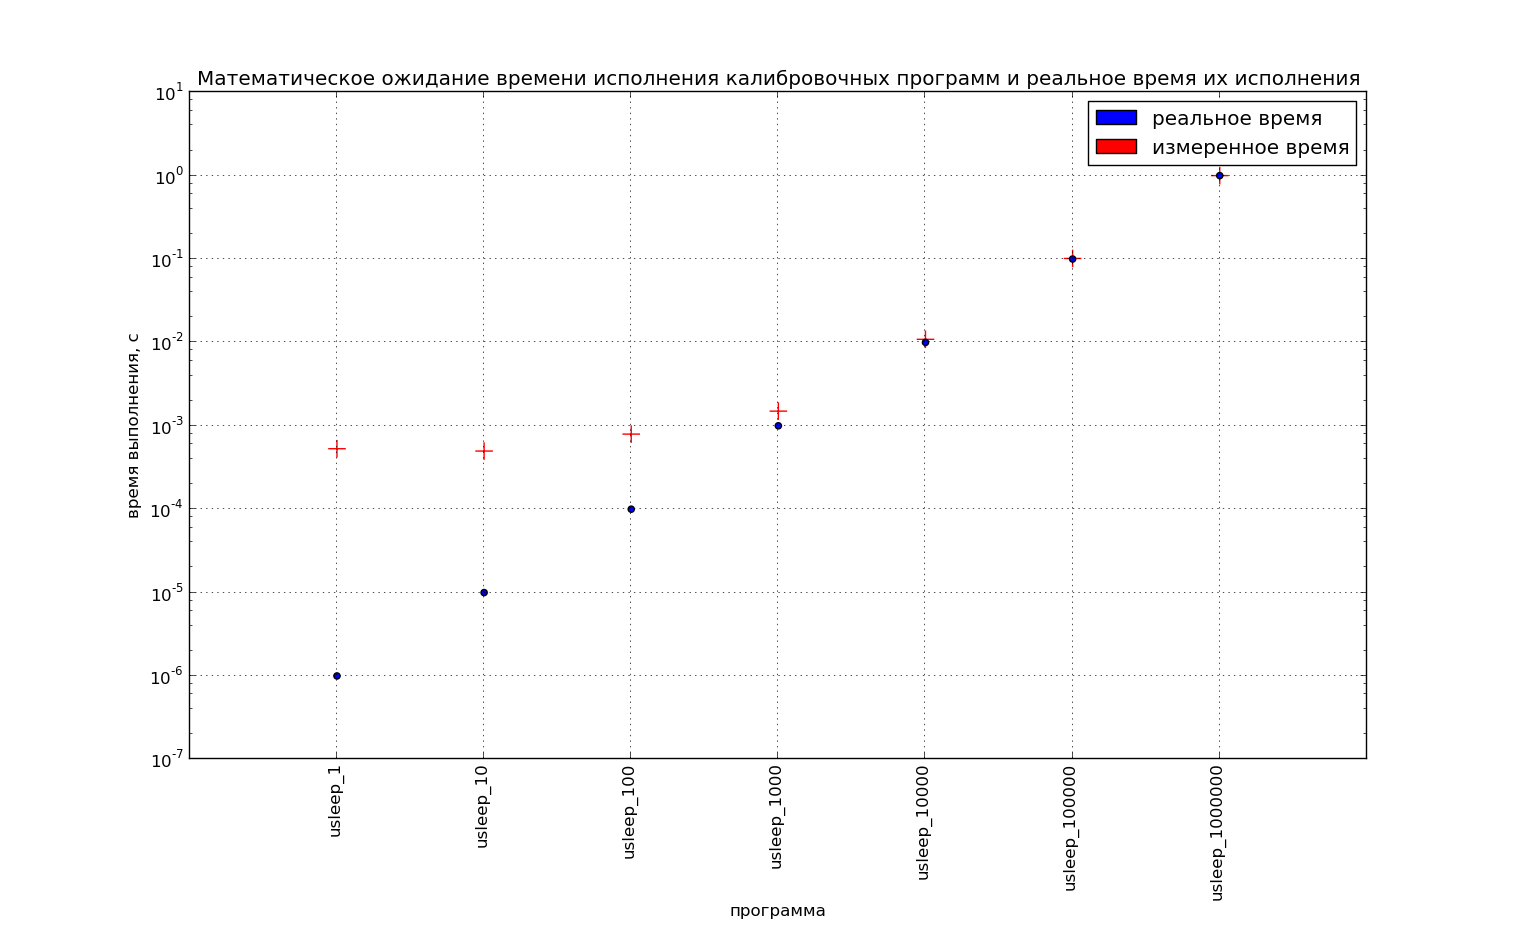
\includegraphics[width=1\linewidth]{calibration-offset}}
    \caption{График измеренного и реального времени исполнения семейства калибровочных программ с учётом накладных расходов}
    \label{img:calibration-offset}
\end{figure}

Далее на рис. \ref{img:default_calibration} приведён текстовый вывод из инструментария результата описанного эксперимента с учётом накладных расходов.

\begin{figure}[H]
    \fontsize{10}{12}
    \begin{verbatim}
        Experiment performed:
            Real time: 0.000001
            Measured time: 0.000531
            Relative error: 530.11
        
        Experiment performed:
            Real time: 0.000010
            Measured time: 0.000498
            Relative error: 48.79
        
        Experiment performed:
            Real time: 0.000100
            Measured time: 0.000795
            Relative error: 6.95
        
        Experiment performed:
            Real time: 0.001000
            Measured time: 0.001499
            Relative error: 0.50
        
        Experiment performed:
            Real time: 0.010000
            Measured time: 0.010893
            Relative error: 0.09
        
        Experiment performed:
            Real time: 0.100000
            Measured time: 0.101603
            Relative error: 0.02
        
        Experiment performed:
            Real time: 1.000000
            Measured time: 1.001015
            Relative error: 0.00
    \end{verbatim}
    \caption{Результат работы программы для описанного выше эксперимента.}
    \label{img:default_calibration}
\end{figure}

Таким образом, инструментарий позволяет производить достаточно точное измерение времени (ошибка в пределах 10\%) для программ, исполняющихся 10 мс и более.


\subsection{Серия экспериментов по сравнению компиляторов GCC и LLVM на тестовом наборе Polybench}
\label{series-llvm-vs-gcc}
На рис. \ref{img:gcc-vs-clang} сравнивается время исполнения программ, собранных компиляторами GCC и LLVM соответственно на уровне оптимизации '-O2'. Компилятор на этом уровне оптимизации в подавляющем большинстве случаев генерирует наиболее быстрый код (относительно уровней '-O0' и '-O1').

\begin{figure}[!bH]
    \center{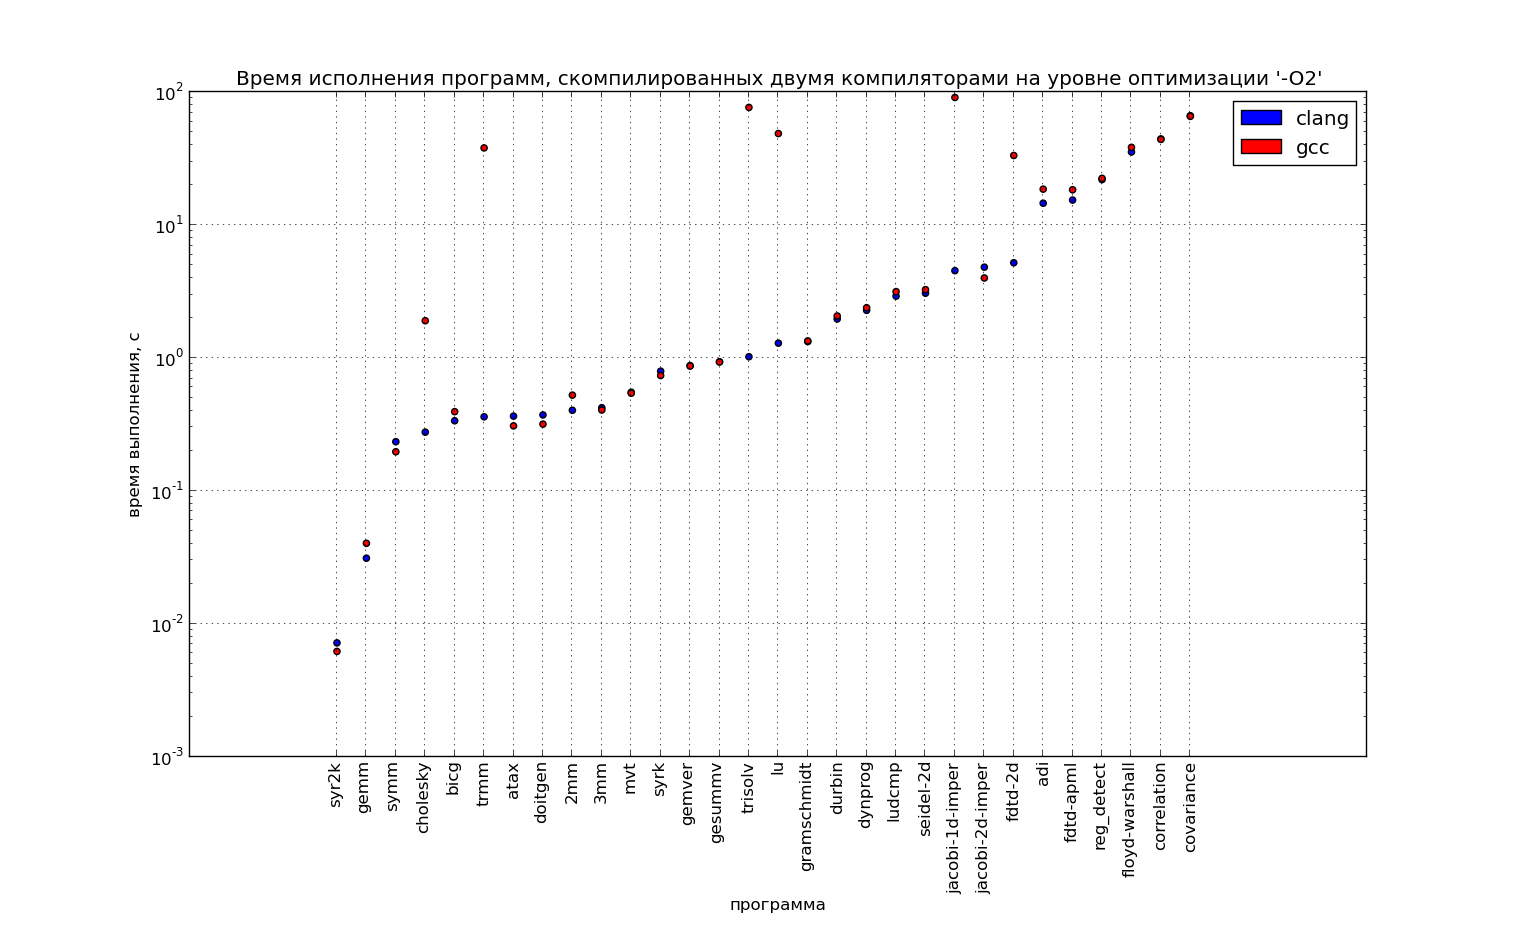
\includegraphics[width=1\linewidth]{gcc-vs-clang}}
    \caption{График времени исполнения программ из набора Polybench для двух компиляторов.}
    \label{img:gcc-vs-clang}
\end{figure}

Как мы видим из графика, на большинстве программ оба компилятора показывают примерно одинаковую производительность. Однако на шести программах компилятор LLVM серьёзно превосходит GCC -- это программы \textit{cholesky, trmm, trisolv, lu, jacobi-1d-imper, fdtd-2d}. Вероятно, LLVM использует лучший векторизатор кода, что оказывает большое влияние в этих специфических случаях. В целом, указанные программы относятся к различным классам -- это программы решения СЛАУ и СДУ. Выяснение конкретных причин этого превосходства выходит за рамки данной работы.

\subsection{Группа серий экспериментов по моделированию и предсказанию производительности программы из набора Polybench на различном аппаратном обеспечении}

Одной из возможностей, предоставляемых инструментарием, является статистический анализ данных серии экспериментов с целью предсказания производительности программ на различном аппаратном обеспечении при различном размере и форме входных данных.

Для этого выберем программу из набора Polybench, которую будем анализировать. Критериями выбора являются факторы, приведённые ниже.
\begin{itemize}
    \item Время исполнения программы при различных размерах и формах входных данных должно быть не слишком велико. Поскольку в рамках серии экспериментов программа должна быть исполнена статистически значимое число раз (по крайней мере 100), мы должны выбрать программу с учётом доступных ресурсов машинного времени и общих ресурсов времени, которое можно потратить на исследование.
    \item Время исполнения программы при различных размерах и формах входных данных должно быть не слишком мало. При уменьшении времени однократного исполнения программы погрешность измерения реального времени исполнения возрастает -- до 50\% при времени однократного исполнения 0,001 с (см. раздел \ref{series-accuracy}). Поэтому мы должны выбрать программу, которая исполняется секунду или более, для достижения оптимальных результатов. При указанном времени исполнения точность измерения времени достигает как минимум 99\% (раздел \ref{series-accuracy}).
\end{itemize}

На основании указанных критериев и данных, полученных в рамках серии экспериментов, описанной в разделе \ref{series-llvm-vs-gcc}, выбираем программу \texttt{symm} в качестве анализируемой.

Мы осуществим три серии экспериментов по моделированию и предсказанию производительности программы \texttt{symm} из набора Polybench. Они перечислены ниже.
\begin{enumerate}
    \item Первая серия экспериментов характеризуется размерами входных данных $M$ (число столбцов обрабатываемой матрицы) и $N$ (число строк обрабатываемой матрицы), задаваемыми по степенному закону $M = N = 2^x, x = [1;12]$. Таким образом, $M = N \in [2;4096]$.
    \item Вторая серия экспериментов характеризуется размерами входных данных $M$ и $N$, задаваемыми случайно из диапазона [2;2048]: $M = N = rand([2;2048])$, где $rand$ -- функция случайного выбора целого числа из указанного диапазона по равномерному закону распределения. Таким образом, $M = N \in [2;2048]$.
    \item Третья серия экспериментов характеризуется размерами входных данных $M$ и $N$, задаваемыми случайно и независимо из диапазона [2;2048]: $M = rand_1([2;2048]), N = rand_2([2;2048])$, где $rand_i, i \in [1;2]$ -- выборки случайного выбора целого числа из указанного диапазона по равномерному закону распределения (в данном случае выбираются два случайных числа). Таким образом, $M, N \in [2;2048]$.
\end{enumerate}

В каждой серии экспериментов производится обучение трёх предсказателей -- \textit{Earth, Random Forest и k-Nearest Neigbour} -- и последующее предсказание производительности программы \texttt{symm} на различных аппаратных платформах и при различных размерах входных данных. Обучение производится на двух различных моделях -- простейшей (включающей всего один признак из набора экспериментальных данных), и более сложной (включающей в себя до пяти признаков из набора экспериментальных данных). Обучение и предсказание на основе экспериментальных данных производится в системе статистической обработки данных с открытым исходным кодом Orange \cite{orange}.

Опишем систему моделирования и предсказания более подробно. Она организована в форме конвейера с ветвлениями. Более подробно система описана в следующем разделе.

\subsubsection{Конвейер статистической обработки данных в системе Orange}
На рисунке \ref{img:series30} изображён конвейер статистической обработки данных в системе Orange. Он имеет такой вид для всех трёх серий экспериментов. Далее мы опишем каждый компонент, используемый в схеме анализа данных, изображённой на указанном рисунке.

\begin{figure}[H]
    \center{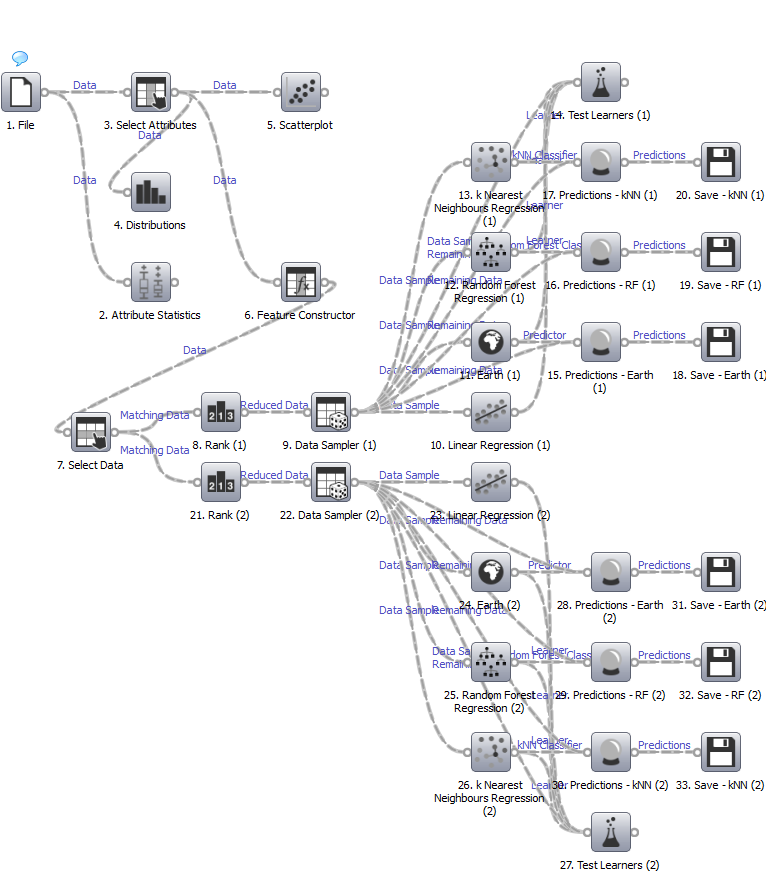
\includegraphics[width=1\linewidth]{series30}}
    \caption{Конвейер обработки данных в системе Orange.}
    \label{img:series30}
\end{figure}

Обработка данных в системе начинается с чтения входных данных в формате CSV из файла -- за это отвечает компонент \texttt{1. File}, находящийся в левом верхнем углу схемы. Отчёт по этому компоненту представлен на рисунке \ref{img:1-File}. Опишем формат входного файла.

\begin{figure}[H]
    \center{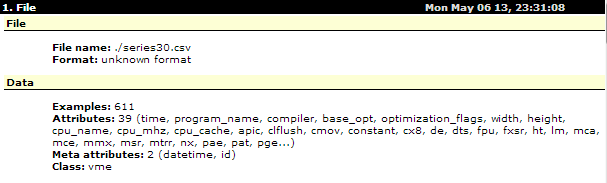
\includegraphics[width=0.7\linewidth]{1-File}}
    \caption{Компонент \texttt{1. File}. Входные данные в файле CSV.}
    \label{img:1-File}
\end{figure}

Входной файл содержит таблицу, в которой столбцы -- это названия свойств эксперимента, полученных во время его выполнения в инструментарии, а строки -- собственно значения этих свойств. Приведём отрывок файла для пояснения его структуры (рисунок \ref{img:series.csv}). Многоточия означают опущенные части файла -- поскольку число свойств достигает сорока, представить файл полностью не представляется возможным ввиду ограниченной ширины страницы. Свойство \texttt{id} также представлено в сокращённом виде -- символы \texttt{..} означают опущенные части строки.

\Rotatebox{90}{
    \begin{minipage}{1.5\linewidth}
        \begin{figure}[H]
            \fontsize{10}{12}
            \begin{verbatim}
id  datetime    time    program_name    compiler    base_opt    optimization_flags  width   height  cpu_name    cpu_mhz cpu_cache   apic ... vme
5104..bd16    2013-04-17 22:25:29 0.0041661978    symm    gcc -O2 None    64  64  Intel(R) Xeon(R) CPU... 2666.76 6144    False ...    False
5104..cc6d    2013-04-17 22:25:14 1.3440570831    symm    gcc -O2 None    256 256 Intel(R) Xeon(R) CPU... 2666.76 6144    False ...    False
5104..d50b    2013-04-17 22:24:57 0.121064496 symm    gcc -O2 None    128 128 Intel(R) Xeon(R) CPU... 2666.76 6144    False ...    False
            \end{verbatim}
            \caption{Отрывок входного файла.}
            \label{img:series.csv}
        \end{figure}
    \end{minipage}
}

Итак, первая строка файла -- названия свойств. \texttt{id} -- уникальный идентификатор эксперимента, \texttt{datetime} -- время его проведения в GMT, \texttt{time} -- время исполнения программы, \texttt{program_name} -- название программы, \texttt{compiler} -- название используемого компилятора, \texttt{base_opt} -- базовый уровень оптимизации программы компилятором, \texttt{optimization_flags} -- дополнительные настройки оптимизации, \texttt{width} -- число столбцов в обрабатываемой матрице, \texttt{height} -- число строк в обрабатываемой матрице, \texttt{cpu_name} -- название процессора, на котором исполнялась программа, \texttt{cpu_mhz} -- частота процессора, \texttt{cpu_cache} -- размер кэша третьего уровня. Все остальные свойства, начиная с \texttt{apic} и заканчивая \texttt{vme} -- двоичные свойства наличия у процессора поддержки определённой возможности, такой как, например, набора инструкций SSE.

Отметим, что пунктирные линии на схеме обозначают передачу данных из одного компонента обработки данных в другой. Схема представляет собой дерево с корнем в узле \texttt{1. File}, причём данные передаются от корня к листьям. Таким образом, из узлов, которые не имеют дочерних, информация дальше не передаётся. Если у узла несколько дочерних узлов, данные передаются от родителя каждому ребёнку данного узла.

Компонент \texttt{2. Attribute Statistics} используется для сбора и показа статистических показателей различных признаков экспериментов, содержащихся в наборе данных -- например, таких, как среднее и медианное значение признака. Выводимые им изображения можно найти в Приложении.

Компонент \texttt{3. Select Attributes} (рисунок \ref{img:3-Select-Attributes}) применяется с целью установления структуры набора данных -- в нём определяется, какие свойства экспериментов являются исходными данными для моделирования (признаками), а какие -- выходными данными (предсказанными значениями). В данном случае все свойства экспериментов, кроме свойства \texttt{time} (время исполнения программы), являются признаками. Свойство \texttt{time} предсказывается моделью.

\begin{figure}[H]
    \center{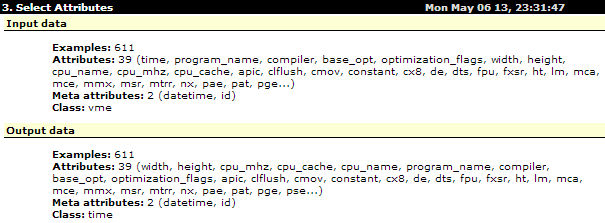
\includegraphics[width=0.9\linewidth]{3-Select-Attributes}}
    \caption{Компонент \texttt{3. Select Attributes}. Определение структуры входных данных.}
    \label{img:3-Select-Attributes}
\end{figure}

Компонент \texttt{4. Distributions} отображает распределения различных атрибутов набора данных. Эти графики можно найти в Приложении.

Компонент \texttt{5. Scatterplot} строит точечные графики зависимости времени исполнения программы от других свойств эксперимента. Пример такого графика можно найти в Приложении. На нём завершается предварительный анализ входных данных.

Компонент \texttt{6. Feature Constructor} используется для создания дополнительного свойства эксперимента из уже присутствующих в наборе данных -- свойства \texttt{size}, определяемого как $size = height \cdot width$ и имеющего смысл агрегированного размера обрабатываемой программой \texttt{symm} матрицы.

Компонент \texttt{7. Select Data} (рисунок \ref{img:7-Select-Data}) может использоваться для фильтрации данных по различным признакам. Например, он может быть использован для удаления из набора данных всех экспериментов, для которых измеренное время исполнения оказалось менее 0,001 с вследствие артефактов измерения. Такая фильтрация может увеличить качество предсказания, поскольку результаты, которые очевидно являются шумом, удаляются из набора данных. Однако, в конечных версиях рассмотренных моделей данный компонент не был задействован, поскольку он требует тонкой настройки и снижает степень автоматизации моделирования.

\begin{figure}[H]
    \center{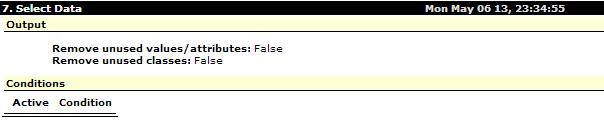
\includegraphics[width=0.9\linewidth]{7-Select-Data}}
    \caption{Компонент \texttt{7. Select Data}. Выбор данных из набора.}
    \label{img:7-Select-Data}
\end{figure}

На этом предварительная обработка данных завершается и начинается собственно построение модели. Компоненты под номерами с 8 по 20 и с 20 по 33 полностью аналогичны. Они представляют собой две ветви конвейера, в одной из которых (с компонентами 8-20) используется простейшая модель на основе единственного признака, а в другой (с компонентами 20-33) -- более сложная модель на основе четырёх или пяти признаков.

Опишем обе ветви конвейера.

Компонент \texttt{8. Rank (1)} (рисунок \ref{img:8-Rank-1}) и его аналог \texttt{21. Rank (2)}  выбирает $S$ наиболее значимых признаков набора данных, при этом $S = 1$ для компонента 8 и $S = 4$ или $S = 5$ для компонента 21. Выбор $S = 4$ или $S = 5$ зависит от результата работы алгоритма выделения важных признаков и для первой и второй серий экспериментов $S = 4$, а для третьей -- $S = 5$.

\begin{figure}[H]
    \center{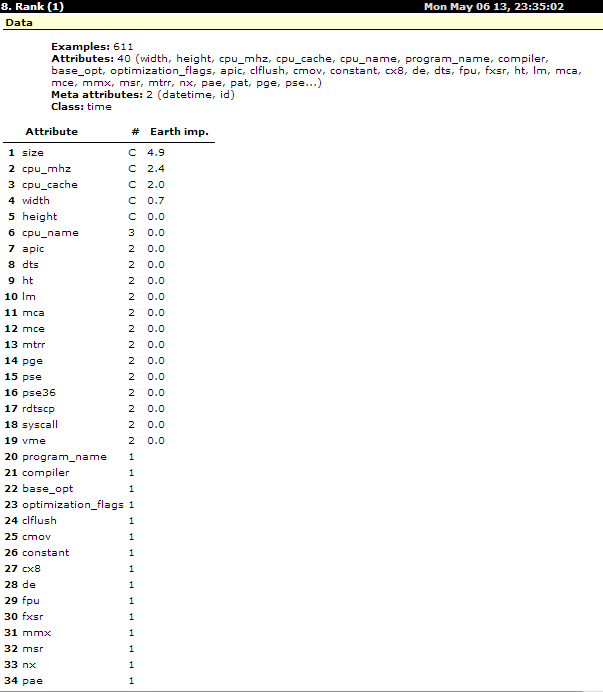
\includegraphics[width=0.9\linewidth]{8-Rank-1}}
    \caption{Компонент \texttt{8. Rank (1)}. Выбор признаков.}
    \label{img:8-Rank-1}
\end{figure}

Компоненты \texttt{9. Data Sampler (1)} и \texttt{22. Data Sampler (2)} производят случайный отбор 70\% данных из набора в учебный набор, а остальных 30\% -- в проверочный набор данных. Это необходимо для проведения перекрёстной проверки, которая в данном случае является одно-проходной ввиду ограниченных ресурсов времени и невысокой степени автоматизации осуществления перекрёстной проверки в системе Orange. При этом компонент 9 работает с моделью, построенной на основе единственного признака, который был оценён, как наиболее важный, компонентом 8. Компонент 22 работает с моделью на основе четырёх или пяти признаков, наиболее важных по результатам работы компонента 21. Далее мы не будем останавливаться на различиях моделей в ветках (8-20) и (20-33).

\begin{figure}[H]
    \center{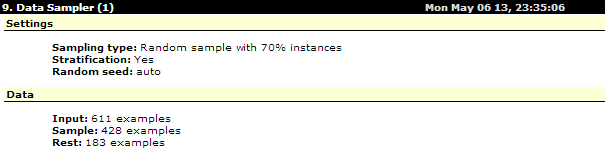
\includegraphics[width=0.9\linewidth]{9-Data-Sampler-1}}
    \caption{Компонент \texttt{9. Data Sampler (1)}. Отбор объектов в обучающую и проверочную выборки.}
    \label{img:9-Data-Sampler-1}
\end{figure}

Компоненты \texttt{10. Linear Regression (1)} и \texttt{23. Linear Regression (2)} строят модели линейной регрессии на основе экспериментальных данных. Эти модели являются образцовыми. Это значит, что качество результатов данных моделей является нижней границей для качества результатов любых других моделей. Поскольку линейная регрессия является простейшим предсказателем, рассмотрение моделей, которые дают результаты хуже, чем линейная регрессия, не имеет смысла. Модели из компонентов 10 и 23 передаются в компоненты 14 и 27 соответственно, где те сравниваются с другими предсказателями по нескольким метрикам (см. ниже).

Компоненты \texttt{11. Earth (1), 12. Random Forest Regression (1), 13. k Nearest Neighbours Regression (1)} и \texttt{11. Earth (2), 12. Random Forest Regression (2), 13. k Nearest Neighbours Regression (2)} являются модулями построения предсказателей \textit{Earth, Random Forest} и \textit{kNN} для ветвей (8-20) и (20-33) соответственно.

\begin{figure}[H]
    \center{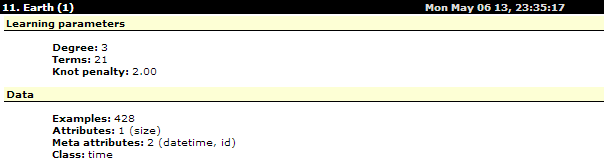
\includegraphics[width=0.9\linewidth]{11-Earth-1}}
    \caption{Компонент \texttt{11. Earth (1)}. Предсказатель Earth для модели с одним признаком.}
    \label{img:11-Earth-1}
\end{figure}

\begin{figure}[H]
    \center{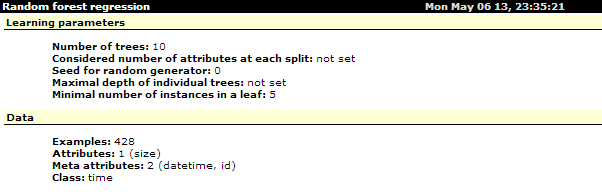
\includegraphics[width=0.9\linewidth]{12-RF-1}}
    \caption{Компонент \texttt{12. Random Forest (1)}. Предсказатель Random Forest для модели с одним признаком.}
    \label{img:12-RF-1}
\end{figure}

\begin{figure}[H]
    \center{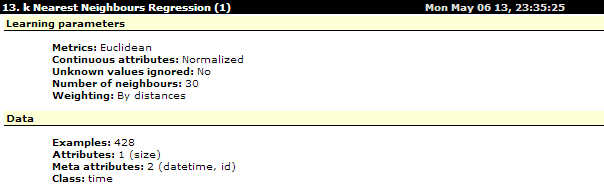
\includegraphics[width=0.9\linewidth]{13-kNN-1}}
    \caption{Компонент \texttt{13. kNN (1)}. Предсказатель k Nearest Neighbours для модели с одним признаком.}
    \label{img:13-kNN-1}
\end{figure}

\begin{figure}[H]
    \center{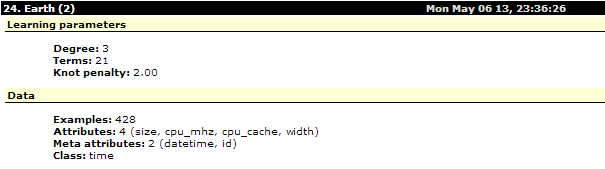
\includegraphics[width=0.9\linewidth]{24-Earth-2}}
    \caption{Компонент \texttt{24. Earth (2)}. Предсказатель Earth для модели с четырьмя признаками.}
    \label{img:24-Earth-2}
\end{figure}

\begin{figure}[H]
    \center{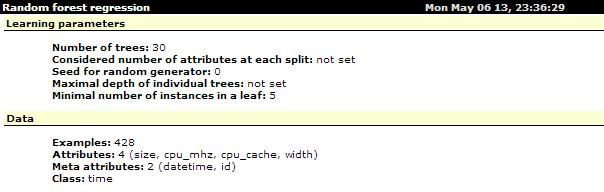
\includegraphics[width=0.9\linewidth]{25-RF-2}}
    \caption{Компонент \texttt{25. Random Forest (2)}. Предсказатель Random Forest для модели с четырьмя признаками.}
    \label{img:25-RF-2}
\end{figure}

\begin{figure}[H]
    \center{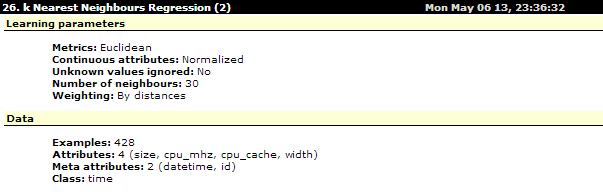
\includegraphics[width=0.9\linewidth]{26-kNN-2}}
    \caption{Компонент \texttt{26. kNN (2)}. Предсказатель k Nearest Neighbours для модели с четырьмя признаками.}
    \label{img:26-kNN-2}
\end{figure}

После обучения предсказателей их параметры передаются в компоненты сравнения качества результатов \texttt{14. Test Learners (1)} и \texttt{27. Test Learners (2)}. Кроме этого, они используются для построения предсказаний в компонентах \texttt{15. Predictions - Earth (1), 16. Predictions - RF (1), 17. Predictions - kNN (1)} и {28. Predictions - Earth (2), 29. Predictions - RF (2), 30. Predictions - kNN (2)} соответсвенно.

\begin{figure}[H]
    \center{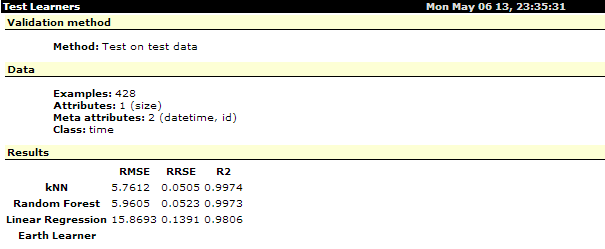
\includegraphics[width=0.9\linewidth]{14-Test-Learners-1}}
    \caption{Компонент \texttt{26. Test Learners (2)}. Сравнение предсказателей для модели с одним признаком.}
    \label{img:14-Test-Learners-1}
\end{figure}

\begin{figure}[H]
    \center{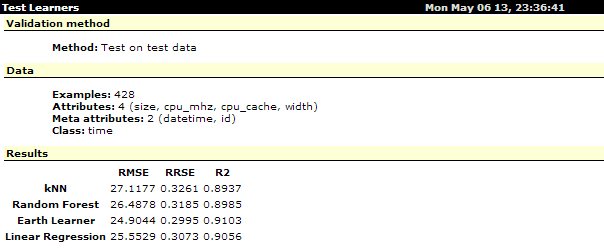
\includegraphics[width=0.9\linewidth]{27-Test-Learners-2}}
    \caption{Компонент \texttt{27. Test Learners (2)}. Сравнение предсказателей для модели с четырьмя признаками.}
    \label{img:27-Test-Learners-2}
\end{figure}

После построения предсказаний, они сохраняются в файлах CSV с помощью компонентов \texttt{18. Save - Earth (1), 19. Save - RF (1), 20. Save - kNN (1)} и \texttt{31. Save - Earth (2), 32. Save - RF (2), 33. Save - kNN (2)} в формате, аналогичном формату исходного файла, загруженного компонентом \texttt{1. File}.

Рассмотрим результаты выполнения этих серий экспериментов и моделирования производительности программы \texttt{symm} в каждом случае.

\subsubsection{Серия экспериментов №1}

Результаты сравнения предсказателей показаны на рисунках~\ref{img:series30-Test-Learners-1}~и~\ref{img:series30-Test-Learners-2}.

\begin{figure}[H]
    \begin{center}
            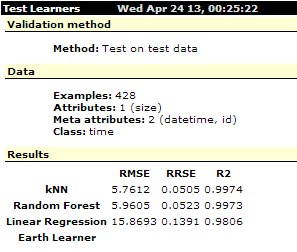
\includegraphics[scale=0.75]{series30-Test-Learners-1}
            \caption{Сравнение предсказателей для модели с одним признаком.} %% подпись к рисунку
            \label{img:series30-Test-Learners-1} %% метка рисунка для ссылки на него
    \end{center}
\end{figure}

\begin{figure}[H]
    \begin{center}
            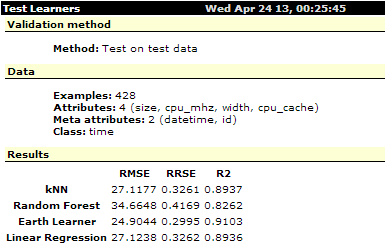
\includegraphics[scale=0.75]{series30-Test-Learners-2}
            \caption{Сравнение предсказателей для модели с четырьмя признаками.}
            \label{img:series30-Test-Learners-2}
    \end{center}
\end{figure}